%-*- coding: UTF-8 -*-
\documentclass[hyperref,a4paper,UTF8]{ctexart}
\usepackage{geometry}
\usepackage[format=hang,font=small,textfont=it]{caption}
\usepackage[nottoc]{tocbibind}
\usepackage{tocloft}
\usepackage{hyperref}
\usepackage{graphicx}
\usepackage{mathtools}
\usepackage{longtable}
\usepackage{array}
\usepackage{enumitem}
\usepackage{eqexpl}

\geometry{a4paper,centering}
\renewcommand\cftdot{·}
\renewcommand{\cftdotsep}{0}
\bibliographystyle{plain}

\begin{document}
\begin{titlepage}
    \vspace*{\fill}
    \begin{center}
        \normalfont
        %\underline{\_\_\_\_\_\_\_\_\_\_\_\_\_\_\_\_\_\_\_\_\_\_\_\_\_\_\_\_\_\_\_\_\_\_\_\_\_}

        {\Huge\bfseries 2021\mbox{年深圳杯竞赛}B\mbox{题}}

        \bigskip
        %\setlength{\lineskiplimit}{0.2bp}\setlength{\lineskip}{0.2bp}\linespread{0.2}\selectfont
        {\Huge\bfseries 火星探测器着陆控制方案}

        %\underline{\_\_\_\_\_\_\_\_\_\_\_\_\_\_\_\_\_\_\_\_\_\_\_\_\_\_\_\_\_\_\_\_\_\_\_\_\_}

        \bigskip
        \bigskip
        \bigskip
        \bigskip
        \bigskip
        \bigskip
        \linespread{1.3}\selectfont
        {\Large\heiti 队员:}
        \Large\kaishu
        \begin{tabular}[t]{@{}c}
            朱旭 \\杨雪桐\\吕义春
        \end{tabular}

        \medskip
        {\Large\heiti 指导教师:}
        \Large\kaishu
        \begin{tabular}[t]{@{}c}
            马龙
        \end{tabular}

        \medskip
        \bigskip
        \bigskip
        \normalfont
        2021年8月
    \end{center}
    \vspace{\stretch{3}}
    \begin{center}
        山东大学
    \end{center}
\end{titlepage}
\begin{abstract}
    \stepcounter{page}
    \addcontentsline{toc}{section}{摘要}
    2021年5月15日,我国天问一号探测器成功着陆火星。对我国有着重大的意义。探测器从地球发射到登陆
    火星这一过程中的每一步都困难重重,需要仔细的研究推演才能成功。本文以天问一号为例来研究探测器
    从火星同步轨道出发到探测器在火星地表上方悬停的过程(以下简称着陆过程)。为了解决问题,我们构
    建了一个用来描述探测器着陆过程的数学模型,用来模拟探测器的运动过程。为了高效地模拟该过程,我
    们先提前将各个影响因素分别计算,再观测其影响。经过筛选后,把那些微不足道的影响因素都剔除出去,
    只留下影响比较明显的一些因素。除此之前,又通过查询资料得到一些动作执行的条件,以此来对模型中
    的一些变量进行限制。在此基础上,通过计算求解来得到不同目的下的最优解。

    虽然目前国内有不少关于火星着陆的论文,但是聚焦于这一过程的论文并不多,大多数是研究一个更加精
    细的问题。本文正是基于这些论文来进行进一步的探究。\par
    \bigskip
    \bigskip
    \noindent
    \textbf{关键词:} 火星探测;蒙特卡洛法;退火模拟法
\end{abstract}
\newpage
\tableofcontents
\newpage
\section{问题重述与分析}
\subsection{问题背景}
探索外太空、解开外星的谜团一直以来是人类的梦想。从古至今人类不曾在这崎岖不平的探索道路中止步。为此,
人类耗费了大量精力财力。2020年,我国发射了托举着“天问一号”的长征五号运载火箭。2021年5月,天问一号
巡视器成功着陆于火星,中国成为了继美国之后全世界第二个成功登陆火星的国家,这意味着我国的航天实力又
提升至了一个新高度。
\subsection{问题重述}
新华社北京 5 月 15 日电:2021 年 5 月 15 日 7 时 18 分,中华人民共和国天问一号探测器成功着陆于
火星乌托邦平原南部预选着陆区,我国首次火星探测任务着陆火星取得成功。中共中央总书记、国家主席、中
央军委主席习近平致贺电,代表党中央、国务院和中央军委,向首次火星探测任务指挥部并参加任务的全体同
志致以热烈的祝贺和诚挚的问候。习近平主席在贺电中指出:%
\textbf{天问一号探测器着陆火星,迈出了我国星际探测征程的重要一步,实现了从地月系到行星际的
    跨越,在火星上首次留下中国人的印迹,这是我国航天事业发展的又一具有里程碑意义的进展。你们勇于挑
    战、追求卓越,使我国在行星探测领域进入世界先进行列,祖国和人民将永远铭记你们的卓越功勋!}

本题聚焦于探测器从火星同步轨道出发到探测器在火星地表上方悬停的过程(以下简称着陆过程),要求参赛队
收集有关天问一号探测器的音像和文字等公开资料,建立数学模型,研究如下问题:
\begin{enumerate}
    \item 确定探测器着陆过程时间最短的操控方案(包括环绕器与着陆巡视器分离、阻尼伞打开、发动机系统
          点火等时间,以及发动机系统运行方案);
    \item 对给定的着陆过程时间,确定消耗能量最少的操控方案;
    \item 如果希望探测器着陆过程与公开的音像和文字资料尽量一致,如何设计操控方案。
\end{enumerate}
\subsection{问题分析}
天问一号探测器从火星同步轨道出发到在火星地表上方悬停主要有六个阶段:两器分离、进入大气、超音速开伞、
大底分离、背罩分离、悬停成像。

针对问题一,因为不控制探测器落点,所以可以忽略火星的自转以及只考虑一个平面内的运动,所以以探测器降落
火星的椭圆轨道中心为原点建立平面直角坐标系。
\section{模型建立}
\subsection{模型假设}
\subsubsection{降落轨道假设}
假设火星为一质量均匀分布的规则球体。由于不控制探测器在火星上的具体落点,所以可以忽略火星的自转。
我们只考虑探测器和火星在一个平面内的运动,所以只需建立一个如图 \ref{pic:syt0} 平面直角坐
标系即可。为了便于探测器的运行轨道的描述和计算,我们以探测器向火星降落的椭圆轨道的中心为原
点,从轨道中心到火星的方向为 x 轴正方向建系。以此坐标系来讨论从同步轨道出发到两器分离的情况。
\begin{figure}[hb]
    \centering
    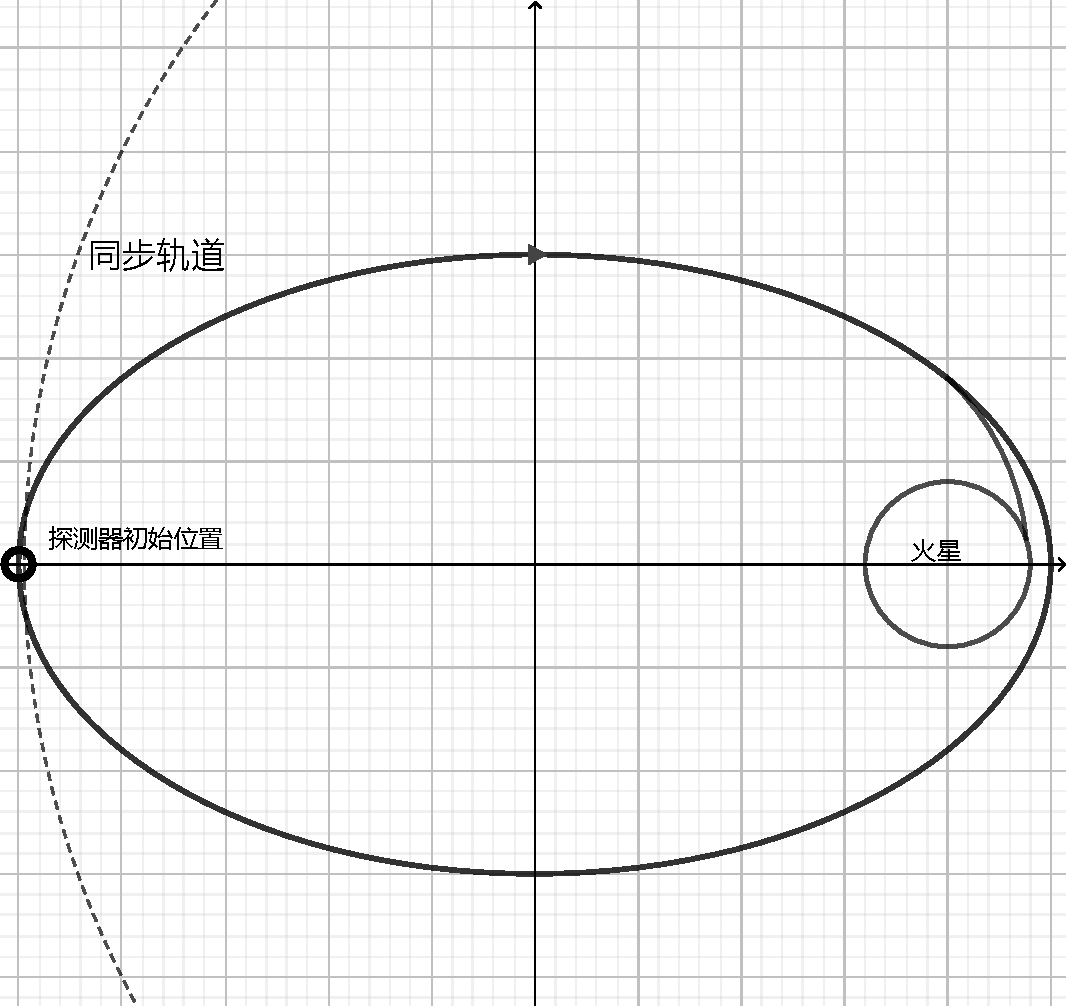
\includegraphics[scale=0.5]{建系示意图0.pdf}
    \caption{平面直角坐标系示意图}
    \label{pic:syt0}
\end{figure}
\subsubsection{火星大气模型假设}
目前公开的火星大气数据库分别是欧洲的 MCD 和美国的 Mars-GRAM。但是这些数据库数据量大,不适合直接
进行计算。所以我们用其数据拟合得到的指数模型来描述大气。

我们假设火星大气层的温度相对海拔呈线性变化,压力随着海拔降低呈指数型增长。得到
的压力-温度拟合公式为:
\[
    \begin{dcases}
        T = -31 - 0.000998 · H
        \quad
        (T\text{的单位为}^\circ C\text{,}H\text{的单位为}m) \\
        P = 0.699 · e^{-0.00009 · H}
        \quad
        (P\text{的单位为}kPa)
    \end{dcases}
\]
而大气的密度可由以下式子得出:
\[
    \rho = \frac{P}{(T + 273.15)\times 0.1921}
\]
除此之外,我们还可以根据声速的计算式来计算火星上的声速:
\[
    v_c = \sqrt{\kappa RT / M}
\]
上式中,$\kappa $ 为大气绝热指数,在火星上取 $1.29$。$R$ 为通用气体常数,取
$8.314472J/(K·mol)$。$T$ 为大气绝对温度,单位为 $K$。$M$ 为大气平均分子摩尔质量,火星
上取 $43.34\times 10^{-3}kg/mol$。
\subsection{符号说明}
\begin{longtable}[h]{|c|p{10cm}|}
    \hline
    \bfseries 符号     & \multicolumn{1}{c|}{\bfseries 说明}                    \\
    \endhead
    \hline
    \bfseries 符号     & \multicolumn{1}{c|}{\bfseries 说明}                    \\
    \endfirsthead
    \multicolumn{2}{c}{\itshape 接下一页表格······}
    \endfoot
    \endlastfoot
    \hline
    $a$                & 椭圆轨道半长轴                                         \\
    \hline
    $b$                & 椭圆轨道半短轴                                         \\
    \hline
    $c$                & 椭圆轨道的焦距的{}$\frac{1}{2}$                        \\
    \hline
    $h$                & 两器分离时的位置到火星表面的距离                       \\
    \hline
    $h_1$              & 远火点到火星表面的距离                                 \\
    \hline
    $h_2$              & 近火点到火星表面的距离                                 \\
    \hline
    $h_3$              & 巡视器打开降落伞时高度                                 \\
    \hline
    $h_4$              & 巡视器大底分离时高度                                   \\
    \hline
    $h_5$              & 巡视器背罩分离时高度                                   \\
    \hline
    $h_6$              & 巡视器开启发动机时高度                                 \\
    \hline
    $r$                & 火星半径                                               \\
    \hline
    $x_0$              & 两器分离时的横坐标                                     \\
    \hline
    $y_0$              & 两器分离时的纵坐标                                     \\
    \hline
    $x$                & 椭圆轨道上任意一点横坐标                               \\
    \hline
    $y$                & 椭圆轨道上任意一点的纵坐标                             \\
    \hline
    $T_0$              & 火星同步轨道的周期,为$24\times 60\times 60 + 37\times
    60 + 22.7s$                                                                 \\
    \hline
    $T_1$              & 椭圆轨道上的周期                                       \\
    \hline
    $M$                & 火星的质量,为$6.4171\times 10^{23}kg$                 \\
    \hline
    $G$                & 引力常量,为$6.67\times 10^{-11}N·m^2/kg^2$            \\
    \hline
    $S$                & 探测器与火星的连线从远火点到两器分离时扫过的面积       \\
    \hline
    $S_1$              & 椭圆轨道的面积                                         \\
    \hline
    $S_{\text{floor}}$ & 大底的底面积,为$2^2·\pi m^2$                          \\
    \hline
    $S_{\text{para}}$  & 降落伞打开后的面积,为$200m^2$                         \\
    \hline
    $v_0$              & 巡视器两器分离时的速度                                 \\
    \hline
    $t_1$              & 从同步轨道到两器分离的时间                             \\
    \hline
    $t_2$              & 从两器分离到打开降落伞的时间                           \\
    \hline
    $t_3$              & 从降落伞打开到大底分离的时间                           \\
    \hline
    $t_4$              & 从大底分离到背罩分离的时间                             \\
    \hline
    $t_5$              & 从背罩分离到悬停成像的时间                             \\
    \hline
    $t_6$              & 巡视器悬停成像花费的时间                               \\
    \hline
    $m$                & 巡视器的质量,为 $1285kg$                              \\
    \hline
    $m_{\text{floor}}$ & 大底的质量,为 $89.6kg$                                \\
    \hline
    $m_{\text{para}}$  & 降落伞的质量,为 $38kg$                                \\
    \hline
    $m_{\text{hide}}$  & 背罩的质量,为 $245.3kg$                               \\
    \hline
\end{longtable}
\subsection{开始建立}
先来讨论第一阶段---两器分离阶段。探测器先从同步轨道上减速变轨到椭圆轨道。当探测器飞行到近日点
附近时,进行两器分离。环绕器继续绕轨道飞行,着陆巡视器继续向火星降落,脱离了之前的轨道。显然可得:
\[
    \begin{dcases}
        \frac{x^2}{a^2} + \frac{y^2}{b^2} = 1 ; \\
        c^2 = a^2 - b^2;                        \\
        a + c = h_1 + r;                        \\
        a - c = h_2 + r.                        \\
    \end{dcases}
\]
解上面的方程组可得:
\[
    \begin{dcases}
        a = (h_1 + h_2 + 2·R) / 2; \\
        b = \sqrt{a^2 - c^2};      \\
        c = (h_1 - h_2) / 2.       \\
    \end{dcases}
\]

\noindent 根据几何关系及开普勒定律可得:

\[
    \begin{dcases}
        x_0 = \frac{a^2}{c} - \frac{a(h + r)}{c}; \\
        y = \sqrt{b^2 - \frac{b^2}{a^2}x^2};      \\
        S = \int_{-a}^{x^0} y \,dx                \\
        S_1 = \pi · a · b                         \\
        t_1 = \frac{S}{S_1} · T_1
    \end{dcases}
\]
在迭代过程中得到不同的 $h_2$ 和 $h$ 对应的巡视器从同步轨道出发到两器分离的时长 $t_1$,
并将 $t_1$ 作为迭代过程量进一步计算。

\medskip
\bigskip
接下来我们开始讨论第二阶段---进入大气阶段。在此阶
段中,巡视器的受力主要为火星对其的重力和空气摩檫力。为了便于研究,将巡视器速度分为相对于火星
地面的垂直速度与水平速度。此时,需要一个火星地面的基准。假设两器分离的点就位于火星地面的垂直上方,
这就是我们选取的基地面。

为了进行速度的转化,需要先求得原先速度相对于坐标系的斜率 $k$,计算$k$的方法为:
对 $y = \sqrt{b^2 - \frac{b^2}{a^2}x^2}$ 求导,然后代入 $x$ 便得到 $k$。
再由几何关系可以得到,向量 $(x_0 - c, y_0)$ \smallskip 和向量 $(1,k)$ 的夹角 $\theta = \arccos
    \frac{\displaystyle (x_0 - c, y_0)·(1,k)}{\displaystyle\vert (x_0 - c, y_0)\vert \cdot |(1,k)|} $。

\smallskip
可以通过能量守恒求得 $v_0$:
\[
    v_0 = \sqrt{\frac{2\,G\,M\,{\left(R+h_1 \right)}}
        {{\left(R+h\right)}\,{\left(2\,R+h+h_1 \right)}}}
\]

利用 $\theta $ 可求出相对于火星地面的垂直速度 $v_{y0}$ 与水平速度 $v_{x0}$:
\begin{gather*}
    v_{x0} = \cos (\frac{\pi }{2} - \theta ) \cdot v_0 \\
    v_{y0} = \sin (\frac{\pi }{2} - \theta ) \cdot v_0
\end{gather*}

利用动能定理,结合离散化可以得到不同高度之间速度的递推公式:
\[
    \begin{dcases}
        \frac{1}{2}mv_{y_{i + 1}}^2 = \frac{1}{2}mv_{y_{i}}^2 + mg\Delta h -
        \frac{1}{2}\rho _iv_i^2S_{\text{floor}}\Delta h\frac{v_{y_i}}{v_i}                        \\
        \frac{1}{2}mv_{x_{i + 1}}^2 = \frac{1}{2}mv_{x_{i}}^2 + mg\Delta h -
        \frac{1}{2}\rho _iv_i^2S_{\text{floor}}\Delta h\frac{v_{x_i}}{v_i}\frac{v_{x_i}}{v_{y_i}} \\
        v_i^2 = v_{x_i}^2 + v_{y_i}^2
    \end{dcases}
\]
\eqexplSetIntro{\qquad 式中,\ }
\begin{eqexpl}[0mm]
    %\itshape\footnotesize
    \item{$\Delta h$} 离散化中的梯度值
    \item{$\rho$} 针对每个节点高度计算得到的大气密度
\end{eqexpl}
\smallskip

对每个高度段计算时长,并累加得到
$
    \displaystyle t_2=\sum_{i=h}^{h_3}{\displaystyle\frac{\Delta h}{\frac{\displaystyle v_i}
        {\displaystyle 2}+\frac{\displaystyle v_{\textrm{i+1}} }{\displaystyle 2}}}
$

\medskip
\bigskip
下一阶段是超音速开伞阶段。此阶段较进入大气阶段差别不大,不同之处在于巡视器还受到了降落伞带来的空气阻力。
此时得到的递推公式为:
\[
    \begin{dcases}
        \frac{1}{2}mv_{y_{i + 1}}^2 = \frac{1}{2}mv_{y_{i}}^2 + mg\Delta h -
        \frac{1}{2}\rho _iv_i^2(S_{\text{floor}}+S_{\text{para}})\Delta h\frac{v_{y_i}}{v_i} \\
        \frac{1}{2}mv_{x_{i + 1}}^2 = \frac{1}{2}mv_{x_{i}}^2 + mg\Delta h -
        \frac{1}{2}\rho _iv_i^2(S_{\text{floor}}+S_{\text{para}})\Delta h\frac{v_{x_i}}{v_i}
        \frac{v_{x_i}}{v_{y_i}}                                                              \\
        v_i^2 = v_{x_i}^2 + v_{y_i}^2
    \end{dcases}
\]

对每个高度段计算时长,并累加得到
$
    \displaystyle t_3=\sum_{i=h_3}^{h_4}{\displaystyle\frac{\Delta h}{\frac{\displaystyle v_i}
        {\displaystyle 2}+\frac{\displaystyle v_{\textrm{i+1}} }{\displaystyle 2}}}
$

\medskip
\bigskip
下一阶段为大底分离阶段。此阶段与超音速开伞阶段类似,区别在于此阶段没有大底的质量和
对速度有一定的限制。因为在背罩分离时要求速度小于$95m/s$。得到的递推公式为:
\[
    \begin{dcases}
        \begin{split}
            \frac{1}{2}(m-m_{\text{floor}})v_{y_{i + 1}}^2 &=
            \frac{1}{2}(m-m_{\text{floor}})v_{y_{i}}^2 +
            (m-m_{\text{floor}})g\Delta h \\ &\quad - \frac{1}{2}\rho
            _iv_i^2(S_{\text{floor}}+S_{\text{para}})
            \Delta h\frac{v_{y_i}}{v_i}
        \end{split}
        \\
        \begin{split}
            \frac{1}{2}(m-m_{\text{floor}})v_{x_{i + 1}}^2 &=
            \frac{1}{2}(m-m_{\text{floor}})v_{x_{i}}^2 +
            (m-m_{\text{floor}})g\Delta h \\ &\quad -\frac{1}{2}
            \rho _iv_i^2(S_{\text{floor}}+S_{\text{para}})\Delta h
            \frac{v_{x_i}}{v_i}\frac{v_{x_i}}{v_{y_i}}
        \end{split}
        \\
        v_i^2 = v_{x_i}^2 + v_{y_i}^2 \\
        v_i < 95m/s                   \\
    \end{dcases}
\]

对每个高度段计算时长,并累加得到
$
    \displaystyle t_4=\sum_{i=h_4}^{h_5}{\displaystyle\frac{\Delta h}{\frac{\displaystyle v_i}
        {\displaystyle 2}+\frac{\displaystyle v_{\textrm{i+1}} }{\displaystyle 2}}}
$

\medskip
\bigskip
下一阶段是背罩分离阶段。这一阶段同进入大气阶段相似,区别在于没有大底、背罩和降落伞的质量。
可得出的递推公式为:
\[
    \begin{dcases}
        \begin{split}
            \frac{1}{2}(m-m_{\text{floor}}-m_{\text{para}}-m_{\text{hide}})v_{y_{i + 1}}^2 &=
            \frac{1}{2}(m-m_{\text{floor}}-m_{\text{para}}-m_{\text{hide}})
            v_{y_{i}}^2 \\ &\quad + (m-m_{\text{floor}}-m_{\text{para}}-m_{\text{hide}})
            g\Delta h\\ &\quad -\frac{1}{2}\rho _iv_i^2
            S_{\text{floor}}\Delta h\frac{v_{y_i}}{v_i}
        \end{split}
        \\
        \begin{split}
            \frac{1}{2}(m-m_{\text{floor}}-m_{\text{para}}-m_{\text{hide}})v_{x_{i + 1}}^2 &=
            \frac{1}{2}(m-m_{\text{floor}}-m_{\text{para}}-m_{\text{hide}})
            v_{x_{i}}^2 \\ &\quad + (m-m_{\text{floor}}-m_{\text{para}}-m_{\text{hide}})
            g\Delta h \\ &\quad -\frac{1}{2}\rho _iv_i^2S_{\text{floor}}\Delta h
            \frac{v_{x_i}}{v_i}\frac{v_{x_i}}{v_{y_i}}
        \end{split}
        \\
        v_i^2 = v_{x_i}^2 + v_{y_i}^2
    \end{dcases}
\]

对每个高度段计算时长,并累加得到
$
    \displaystyle t_5=\sum_{i=h_5}^{h_6}{\displaystyle\frac{\Delta h}{\frac{\displaystyle v_i}
        {\displaystyle 2}+\frac{\displaystyle v_{\textrm{i+1}} }{\displaystyle 2}}}
$

\medskip
\bigskip
下一阶段是悬停成像阶段,该阶段与背罩分离阶段相似,不同之处在于开启了发动机来减速,受到发动机给的推力。
该阶段得到的拟合公式为:
\[
    \begin{dcases}
        \begin{split}
            \frac{1}{2}(m-m_{\text{floor}}-m_{\text{para}}-m_{\text{hide}})v_{y_{i + 1}}^2 &=
            \frac{1}{2}(m-m_{\text{floor}}-m_{\text{para}}-m_{\text{hide}})
            v_{y_{i}}^2 \\ &\quad + (m-m_{\text{floor}}-m_{\text{para}}-m_{\text{hide}})
            g\Delta h\\ &\quad -\frac{1}{2}\rho _iv_i^2S_{\text{floor}}\Delta h
            \frac{v_{y_i}}{v_i} - 7500N·\frac{\Delta hv_{y_i}}{v_i}
        \end{split}
        \\
        \begin{split}
            \frac{1}{2}(m-m_{\text{floor}}-m_{\text{para}}-m_{\text{hide}})v_{x_{i + 1}}^2 &=
            \frac{1}{2}(m-m_{\text{floor}}-m_{\text{para}}-m_{\text{hide}})
            v_{x_{i}}^2 \\ &\quad + (m-m_{\text{floor}}-m_{\text{para}}-m_{\text{hide}})
            g\Delta h \\ &\quad -\frac{1}{2}\rho _iv_i^2S_{\text{floor}}\Delta h
            \frac{v_{x_i}}{v_i}\frac{v_{x_i}}{v_{y_i}} -
            7500N·\frac{\Delta hv_{x_i}}{v_{y_i}}·\frac{v_{x_i}}{v_i}
        \end{split}
        \\
        v_i^2 = v_{x_i}^2 + v_{y_i}^2
    \end{dcases}
\]

对每个高度段计算时长,并累加得到
$
    \displaystyle t_6=\sum_{i=h_6}^{100m}{\displaystyle\frac{\Delta h}{\frac{\displaystyle v_i}
        {\displaystyle 2}+\frac{\displaystyle v_{\textrm{i+1}} }{\displaystyle 2}}}
$

\smallskip
下面将各个区间段的时间求和得到总时长 $t$,并记录下每段时间的时长和节点高度以便于制定方案:
\[
    t = \sum_{i=1}^{6}t_i
\]
总时长 $t$ ​​在迭代过程中不断比较并更新为最小值,同时更新与之对应的区间时长 $t_i$ 和接点高度 $h_i$:
\begin{gather*}
    t_{\text{ans}}=\min\{{t_{k=1},t_{k=2},...,t_{k=N}}\}\\
    (\text{\itshape 假设总共迭代次数为}N)\\
    h_{\text{ansj}} = h_{k=\text{ans}_i,j}~
    (j=1,2,3,..6)\\
    t_{\text{ansj}} = t_{k=\text{ans}_i,j}~
    (j=1,2,3,..6)
\end{gather*}
\newpage
\nocite{Shiye}
\bibliography{math}
\end{document}